%%%%%%%%%%%%%%%%%%%%%%%%%%%%%%%%%%%%%%%%%%%%%%%%%%%%%%%%%%%%%%%%%%%%%%%%%%%%%
%	e-Yantra, IIT-Bombay

%	Document Author: Abhishek Rathore, G. Harshawardhan
%	Date: 04-July,2016 

%%%%%%%%%%%%%%%%%%%%%%%%%%%%%%%%%%%%%%%%%%%%%%%%%%%%%%%%%%%%%%%%%%%%%%%%%%%%%

\documentclass[11pt,a4paper]{article}

\usepackage{graphicx}
\usepackage{listings}
\usepackage{url}
\usepackage{float}
\usepackage{subcaption}
\title{Tutorial - Re-recognizing the object if it escapes and comes back into the frame.}
\author{e-Yantra Team}
\date{\today}

\begin{document}
	\maketitle
	\newpage
	\tableofcontents
	\newpage
	\section{Objective}
	This tutorial will teach you "How to track the object without errors and How to re-recognize the object if it escapes and comes back into the frame.
	\section{Prerequisites}
	User should have handy knowledge of the following for understanding this tutorial.
	\begin{itemize}
		\item Basics of Python.
		\item Basics of OpenCV.
		\item Basics of Image processing.
		\item CAMShift Algorithm.
	\end{itemize}
	\section{Hardware Requirement}
	\begin{itemize}
		\item A Computer with an internal or external webcam.
	\end{itemize}
	\section{Software Requirement}
	\begin{itemize}
		\item Python 2.7.11
		\item OpenCV 2.4.13 
		\item numpy 1.7.1
		\item \textbf{Note :} These are the versions we were working on while creating this tutorial.
	\end{itemize}
	\section{Theory and Description}
	CAMSHIFT applies traditional mean shift to the backprojection of the appearance model (color histogram) and adds an adaptive region sizing step.
	The tracking phase simply uses CAMSHIFT, and maintains an adaptive histogram distance threshold. When the target object leaves the scene or is occluded, switch to the detection phase, which proceeds as follows.
	\begin{itemize}
	 	\item It backprojects the appearance model to determine the consistency of each pixel with the appearance model.
	 	\item It binarizes the backprojection to eliminate weakly consistent image regions.
	 	\item It generates the connected components using the morpahological filters.
	 	\item It generates a set of candidate regions by eliminating inconsistent connected components. 
	 	\item It finds the most consistent region using histogram comparison between candidate region and target histogram.
	\end{itemize}
	To re-recognize the object, two additions to CAMShift Algorithm are,
	\textbf{Suspend Tracking}\newline 
	CAMSHIFT works extremely well so long as the target appearance remains consistent and distinctive with respect to the background. However, when the target object leaves the scene, is occluded, or impinges a background region with a similar color distribution, the tracking region tends to change rapidly in
	size, growing into background regions or moving to a different location completely. In these situations, it is important to suspend tracking and attempt to re-detect the target object.
	\begin{itemize}
		\item To achieve this, as a first measure it imposes simple constraints on the target detection window’s location and size. If the target object’s estimated size or location changes by an amount inconsistent with robot and target dynamics, clearly, the tracker is lost and needs to be reinitialized.
		\item And before committing to CAMSHIFT’s estimate of the target at time, it verifies the quality of the candidate detection region using an adaptive threshold applied to the dissimilarity between the candidate region’s color histogram and the appearance model. It uses the default OpenCV histogram
		comparison function which returns a distance based on the Bhattacharyya coefficient. The resulting distance varies between 0, for identical histograms, to 1, for non-overlapping histograms. The histogram comparison threshold is computed adaptively. Which contains combination of distance measure’s mean and standard deviation.
	\end{itemize}
	
	\textbf{Target Re-detection}\newline
	While tracking is suspended, on every frame, It executes the target re-detection algorithm. Which is as follows,
	\begin{itemize}
		\item \textbf{Backproject the appearance model}: Backprojection of the appearance model simply means that it generates a new image such that, it will have in general several clusters of pixels with high values, indicating some degree of consistency of the region with object histogram.
		\item \textbf{Binarize likelihood image}: 
	\end{itemize} 
	
	\section{Experiment}
	The Python code is given below
	\lstinputlisting[language=Python]{code.py}
  	
	\section{Exercise}
	Re-detection and tracking of an object  is shown below.
	\begin{figure}[h]
 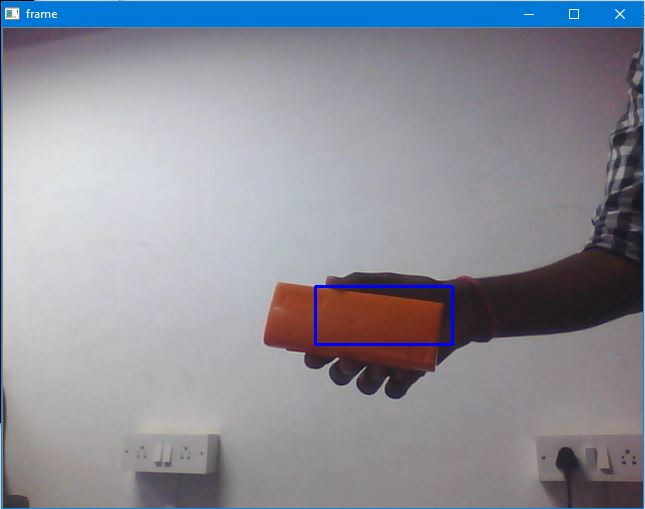
\includegraphics[width=0.9\linewidth, height=10cm]{Image1.jpg}
   \centering
 \caption{Object in the frame}
  \end{figure}
  \begin{figure}[h]
 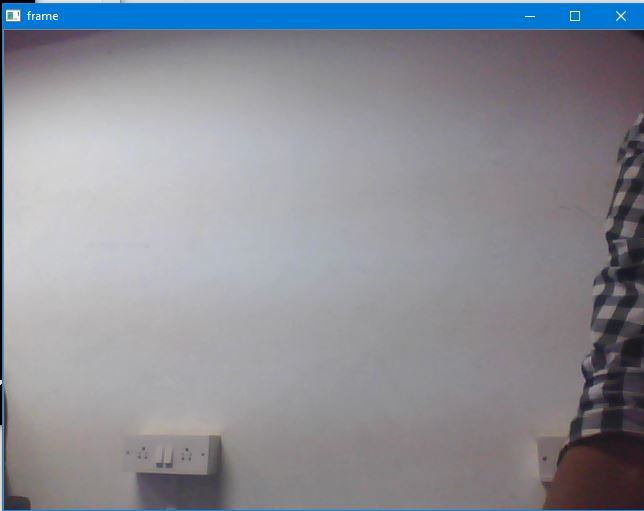
\includegraphics[width=0.9\linewidth, height=6cm]{Image2.jpg}
   \centering
 \caption{Object lost in the frame}
  \end{figure}
  \begin{figure}[h]
 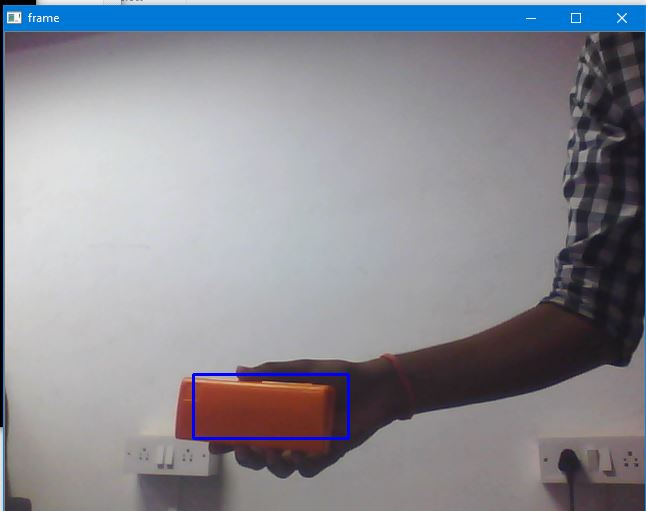
\includegraphics[width=0.9\linewidth, height=6cm]{Image3.jpg}
   \centering
 \caption{Re-detection of object in the frame}
  \end{figure}
	\section{References}
	\begin{enumerate}
			\item \url{https://opencv-python-tutroals.readthedocs.io/en/latest/py_tutorials/py_tutorials.html}

\item \url{http://vgl-ait.org/mdailey/uploads/publication_file/filename/106/Basit-CAMSHIFT.pdf}
   \end{enumerate}
	
\end{document}



